\section{Диффузия мономера в слое полимера}
Ключевая величина, описывающая в процесс диффузии произвольной примеси в слое вещества -- коэффициент диффузии. В настоящее время существуют два основных подхода к определению коэффициента диффузии мономера ММА в слое ПММА. Первый из них основан на использовании теории свободного объема, что позволяет непосредственно определить коэффициент диффузии на основе различных параметров вещества. Второй подход основан на косвенном определении коэффициента диффузии за счет моделирования выхода мономера из слоя ПММА и сравнения результатов моделирования с экспериментальными данными.

\subsection{Теория свободного объема}
Точный расчет коэффициента диффузии возможен на основе теории свободного объема~\cite{Vrentas_free_volume, Zielinski_free_volume}, что требует задания большого числа параметров:
\begin{equation}
	\ln D=\ln \bar{D}_0-\frac{E^*}{\mathrm{R} T}-\left\{\frac{\left(1-\omega_2\right) \hat{V}_1^*+\xi \omega_2 \hat{V}_2^*}{\hat{V}_{\mathrm{FH}} / \gamma}\right\}.
\end{equation}
Здесь $\bar{D}_0$ -- константа, $E^*$ -- энергия на моль частиц примеси, необходимая для преодоления сил притяжения, $R$ -- универсальная газовая постоянная, $T$ -- температура, $\xi$ и $\gamma$ -- параметры, $\hat{V}_1^*$ и $\hat{V}_2^*$ -- удельные объемы вещества и примеси, соответственно, $\hat{V}_{\mathrm{FH}}$ -- средний свободный объем полостей в смеси вещества и примеси, $\omega_2$ -- массовая доля полимера в смеси ($w_p$). Величина $\hat{V}_{\mathrm{FH}} / \gamma$ определяется выражением
\begin{equation}
	\hat{V}_{\mathrm{FH}} / \gamma=\left(1-\omega_2\right)\left(\frac{K_{11}}{\gamma_1}\right)\left(K_{21}+T-T_{\mathrm{g} 1}\right)+\omega_2 \hat{V}_{\mathrm{FH} 2} / \gamma_2,
\end{equation}
где $\left(K_{11} / \gamma_1\right)$ и $\left(K_{21}-T_{\mathrm{g} 1}\right)$ -- параметры примеси, величина $\hat{V}_{\mathrm{FH} 2} / \gamma_2$ описывает вклад полимерной матрицы в средний свободный объем полостей. Эта величина зависит от того, находится система выше или ниже температуры стеклования полимера ($T_{g2}$):
\begin{equation}
	\begin{aligned}
		&\hat{V}_{FH2} =
		\hat{V}_2^0 (T_{g2}) \left[ f_{H2}^{G}+\alpha_2 (T-T_{g2}) \right], & T \geq T_{g2} \\
		&\hat{V}_{FH2} =
		\hat{V}_2^0 (T_{g2})\left[f_{H2}^{G}+(\alpha_2-\alpha_{c2})(T-T_{g2})\right], \hspace{1em} & T<T_{g2}
	\end{aligned}
\end{equation}
В этом выражении $\hat{V}_2^0\left(T_{\mathrm{g} 2}\right)$ -- удельный объем полимера при температуре $T_{g2}$, \linebreak $\alpha_2$ -- коэффициент температурного расширения полимера в состоянии равновесия, $f_{\mathrm{H} 2}^{\mathrm{G}}$ -- доля объема пустот в полимере при температуре $T_{g2}$:
\begin{equation}
	f_{\mathrm{H} 2}^{\mathrm{G}}=\alpha_2 K_{22},
\end{equation}
\begin{equation}
	\alpha_{\mathrm{c} 2}=\frac{1}{T_{\mathrm{g} 2}} \ln \left(\frac{\hat{V}_2^0\left(T_{\mathrm{g} 2}\right)\left(1-f_{\mathrm{H} 2}^{\mathrm{G}}\right)}{\hat{V}_2^0(0)}\right),
\end{equation}
\begin{equation}
	\gamma_2=\frac{\hat{V}_2^0\left(T_{\mathrm{g} 2}\right) \alpha_2}{\left(K_{12} / \gamma_2\right)},
\end{equation}
\begin{equation}
	\hat{V}_1^*=\hat{V}_1^0(0); \hspace{1em} \hat{V}_2^*=\hat{V}_2^0(0),
\end{equation}
где $K_{22}$ и $\left(K_{12} / \gamma_2\right)$ -- параметры модели свободного объема, $\hat{V}_1^0(0)$ и $\hat{V}_2^0(0)$ -- удельные объемы примеси и полимера в состоянии равновесия при $T=0$K. Параметры модели свободного объема для диффузии ММА в слое ПММА приведены в таблице~\ref{table:D_free_volume}~\cite{Tonge_free_volume_parameters}.

\begin{table}[h]
	\centering
	\caption{Константы процессов инициирования активного центра и деполимеризации.}
	\begin{tabular}{l c l}
		\hline \hline
		Параметр & \hspace{4em} & Значение \\ \hline
		$\hat{V}_1^0(0)$, см$^{-1}$ & \hspace{1em} & 0.871 \\
		$\tilde{V}_1^0(0)$, см$^3$ моль$^{-1}$ & \hspace{1em} & 86.9 \\
		$\hat{V}_2^0(0)$, см$^3$ г$^{-1}$ & \hspace{1em} & 0.762 \\
		$\tilde{V}_2^*$, см$^3$ моль$^{-1}$ & \hspace{1em} & 135 \\
		$f_{H2}^{G}$ & \hspace{1em} & 0.00456 \\
		$K_{22}$, К & \hspace{1em} & 80 \\
		$(K_{12} / \gamma_2)$, см$^3$ г$^{-1}$ К$^{-1}$ & \hspace{1em} & 1.28$\times$10$^{-4}$ \\
		$\gamma_2$ & \hspace{1em} & 3.88 \\
		$\alpha_{c2}$, K$^{-1}$ & \hspace{1em} & 2.37$\times$10$^{-4}$ \\
		$\xi_L$ & \hspace{1em} & 0.64 \\
		$\xi$ & \hspace{1em} & 0.58 \\
		$E^*$, Дж моль$^{-1}$ & \hspace{1em} & 0.58 \\
		$\bar{D}_0$, см$^2$ с$^{-1}$ & \hspace{1em} & 1.27$\times$10$^{-3}$ \\
		$(K_{11} / \gamma_1)$, см$^3$ г$^{-1}$ К$^{-1}$ & \hspace{1em} & 6.91$\times$10$^{-4}$ \\
		$(K_{21}-T_{g1})$, К & \hspace{1em} & 72.26 \\
		$\hat{V}_2^0(T_{g2})$, см$^3$ г$^{-1}$ & \hspace{1em} & 0.8754 \\
		$\tilde{V}_c$, см$^3$ моль$^{-1}$ & \hspace{1em} & 311 \\
		\hline \hline
	\end{tabular}
	\label{table:D_free_volume}
\end{table}

Результаты применения модели свободного объема для вычисления коэффициента диффузии ММА в ПММА приведены на рис.~\ref{fig:free_volume_diffusion}

\begin{figure}
	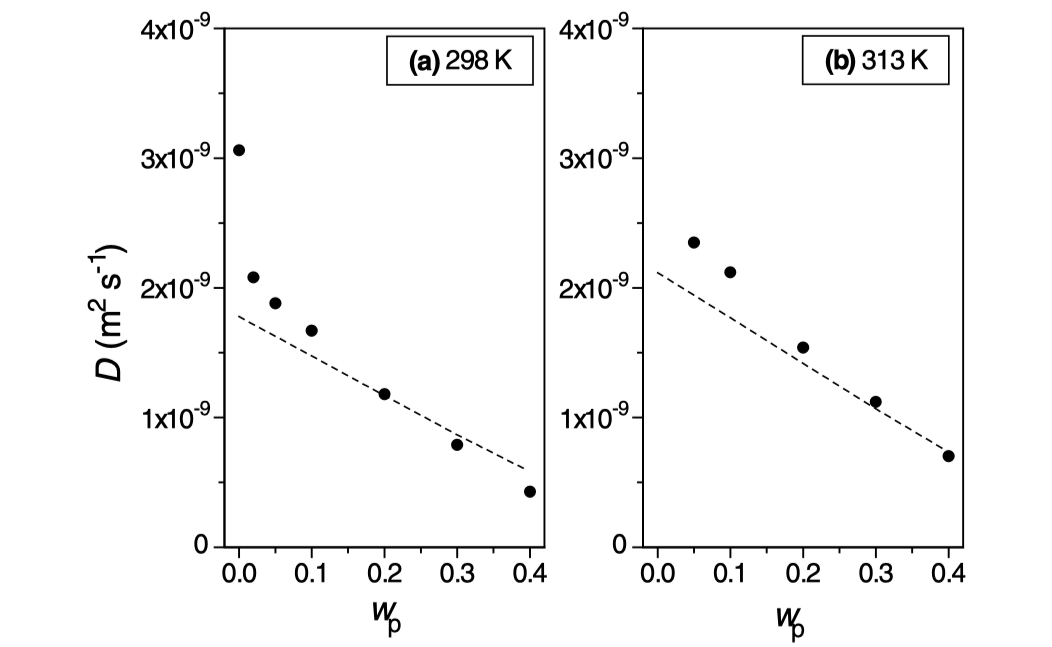
\includegraphics[width=0.9\linewidth]{free_volume_diffusion}
	\caption{Результаты применения модели свободного объема для вычисления коэффициента диффузии ММА в ПММА при 296 К (а) и 313 К (б): пунктирная линия -- рассчитанные значения, точки -- экспериментальные значения~\cite{Griffiths_MMA_PMMA_diffusion}.}
	\label{fig:free_volume_diffusion}
\end{figure}


\subsection{Вычисление коэффициента диффузии на основе модели выхода мономера из слоя полимера}
В работе~\cite{Fragala_3_diffusion} проводилось исследование выхода мономера из слоя ПММА при его экспонировании ионным лучом. В модели процесса деполимеризации ПММА рассматривались процессы инициирования активного центра деполимеризации и распространения активного центра деполимеризации вдоль молекулы:

\begin{equation}
	\begin{aligned}
		&{[\text { Полимер }]_N \stackrel{\text { Экспонирование }}{\longrightarrow}[\text { Полимер }]_{N-m}+[\text { Радикал }]_m,} \\
		&{[\text { Радикал }]_m \stackrel{\text { Деполимеризация }}{\longrightarrow} \text { Мономер }+[\text { Радикал }]_{m-1} .}
	\end{aligned}
\end{equation}
$K_i$ и $K_p$.
Концентрация центров инициирования деполимеризации ($c_I$) описывалась уравнением
\begin{equation}
	\frac{\partial c_I}{\partial t}=K_i f(t)-K_p c_I,
\end{equation}
где $K_i$ и $K_p$ -- константы процессов инициирования и деполимеризации, а функция $f(t)$ описывает режим работы ионного луча:
\begin{equation}
	f(t) = 1 - H(t - t_0),
\end{equation}
где $H(t)$ -- функция Хевисайда,  $t_0$ -- время работы ионного луча.

Образование мономера предполагалось однородным по объему полимера, что позволило описать процесс выхода мономера одномерным уравнением диффузии:
\begin{equation} \label{eq:raduino_diff_eq}
	\frac{\partial c_M}{\partial t}=D\left(\frac{\partial^2 c_M}{\partial z^2}\right)+\beta K_p c_I,
\end{equation}
где $c_M$ -- концентрация мономера, $D$ -- коэффициент диффузии мономера в слое ПММА, считающийся постоянным по всему объему слоя, $\beta$ -- количество мономеров, образующихся при инициирования активного центра деполимеризации.

Уравнение~\ref{eq:raduino_diff_eq} дополнялось начальными и граничными условиями, описывающими беспрепятственный переход мономера через границу ПММА/вакуум, отражение мономера от подложки и его отсутствие до и по истечении большого времени после работы ионного луча, имели вид:
\begin{equation} \label{eq:diff_eq_conditions}
	\begin{aligned}
		&\left.c_M\right|_{z=z_0}=0, \\
		&\left.\frac{\partial c_M}{\partial z}\right|_{z=0}=0, \\
		&\left.c_M\right|_{t=0}=0, \\
		&\lim _{t \rightarrow \infty} c_M=0, \\
		&\lim _{t \rightarrow \infty} c_I=0,
	\end{aligned}
\end{equation}
где $z = 0$ и $z = z_0$ -- границы слоя ПММА.

Решение уравнения~\ref{eq:raduino_diff_eq} с условиями~\ref{eq:diff_eq_conditions} позволило рассчитать поток мономера через границу полимер/вакуум во время работы ионного луча ($t < t_0$):
\begin{equation}
	\begin{aligned}
		J_{+}(t)= & A \beta K_i z_0
		\left[
		1-\frac{8}{\pi^2} \sum_{n=1}^{\infty}
		\frac{1}{(2n-1)^2} \frac{1}{(1-\alpha_n / K_p)} \times \right. \\ & \left.
		\times
		\left(
			\exp (-\alpha_n t)-\frac{\alpha_n}{K_p} \exp (-K_p t)
		\right)
		\right]
	\end{aligned}
\end{equation}
и после выключения ионного луча ($t > t_0$):
\begin{equation}
	\begin{aligned}
		J_{-}(t)= A \beta K_i z_0 \left[
			\frac{8}{\pi^2} \sum_{n=1}^{\infty} \frac{1}{(2 n-1)^2} \frac{1}{\left(1-\alpha_n / K_p\right)}\right. \times \quad \quad \quad \quad \\
	\times \left.
	\left(
	\exp (-\alpha_n t) (\exp (\alpha_n t_0)-1)- \frac{\alpha_n}{K_p}
	\exp (-K_p t) (\exp (K_p t_0)-1)
	\right)
	\right].
	\end{aligned}
\end{equation}

Параметры модели $K_i$, $K_p$ и $\beta$ были подобраны за счет сравнения промоделированной зависимости потока мономера от времени с экспериментальной, их значения приведены в таблице~\ref{table:Ki_Kp_D}.

\begin{figure}
	\begin{minipage}{0.48\textwidth}
		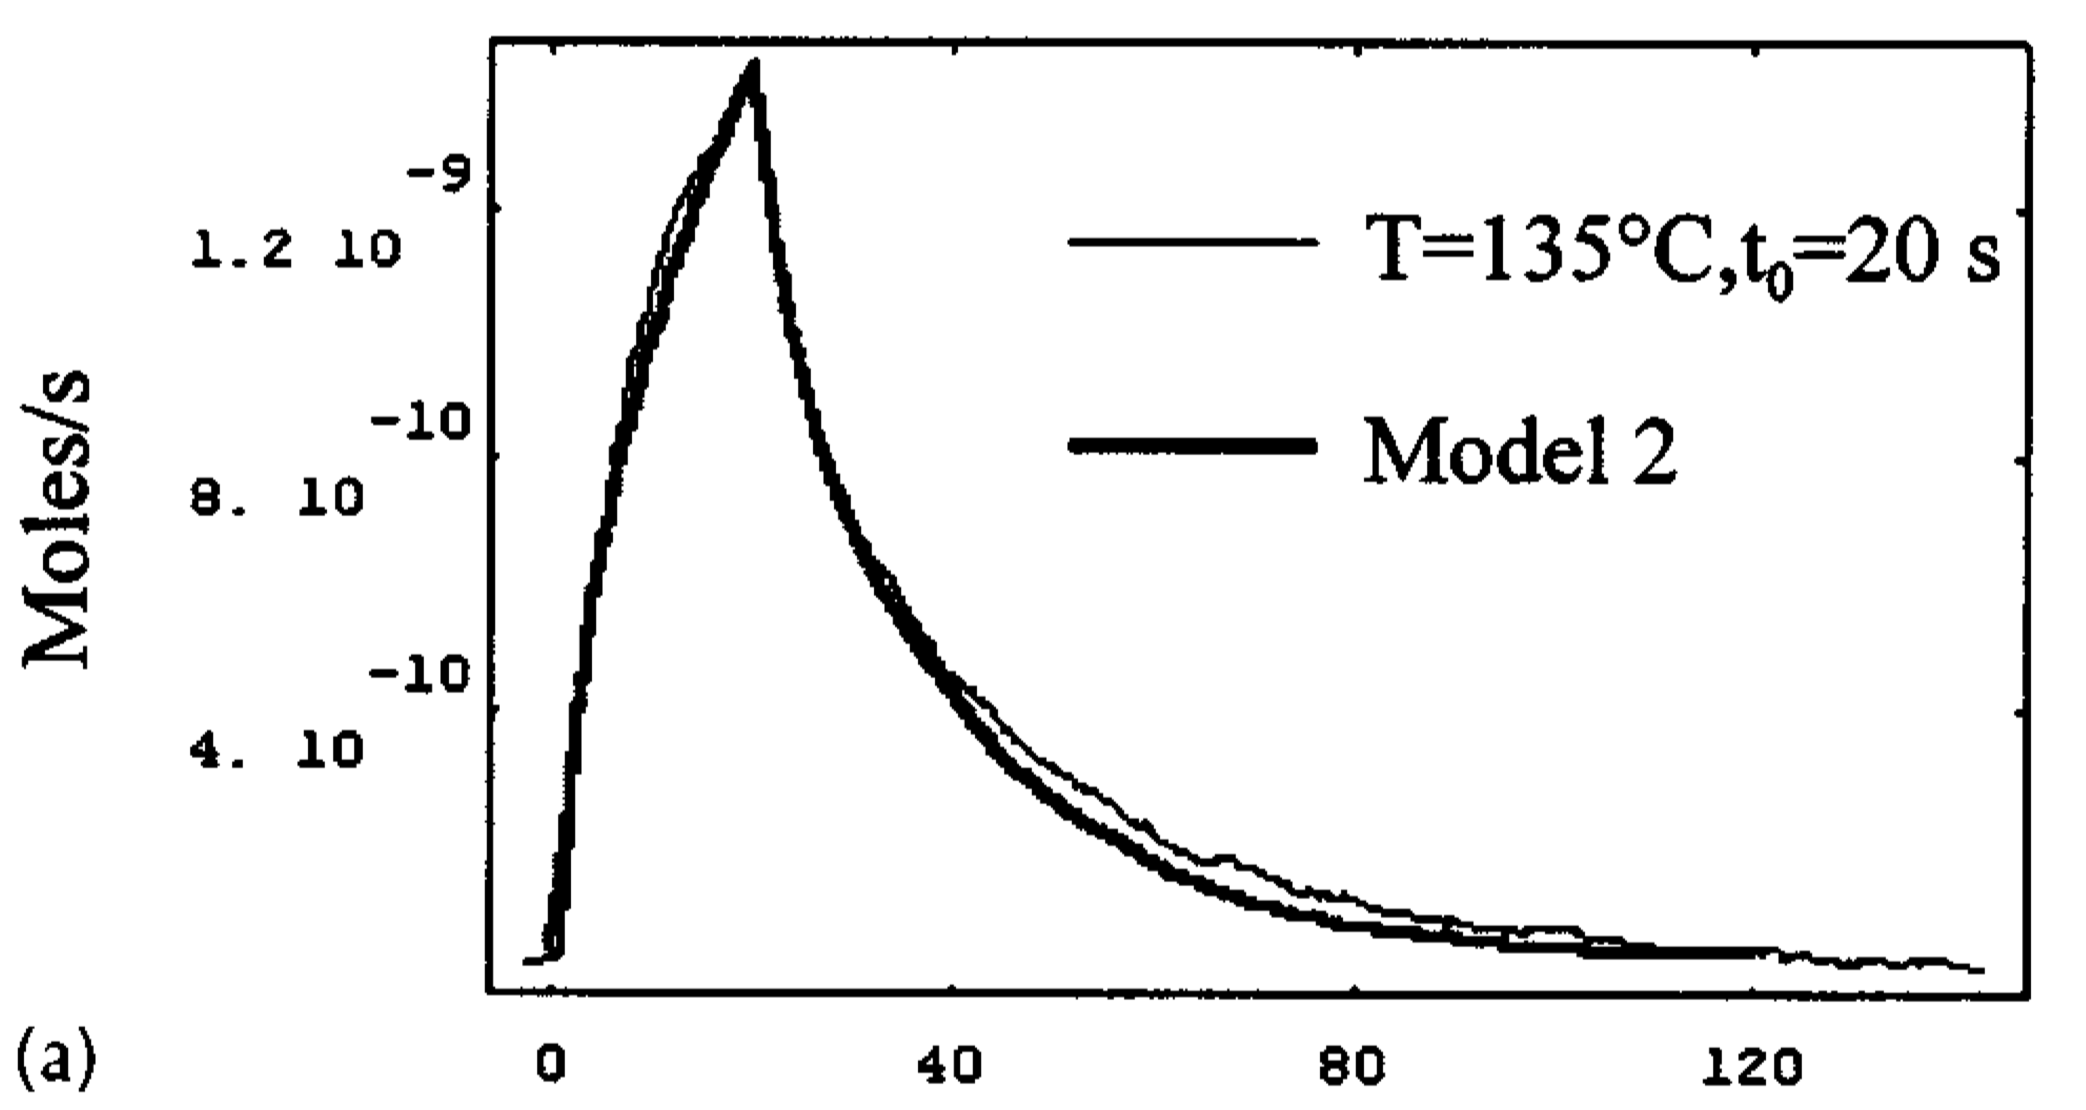
\includegraphics[width=\linewidth]{135_20.png}
	\end{minipage}
	\begin{minipage}{0.48\textwidth}
		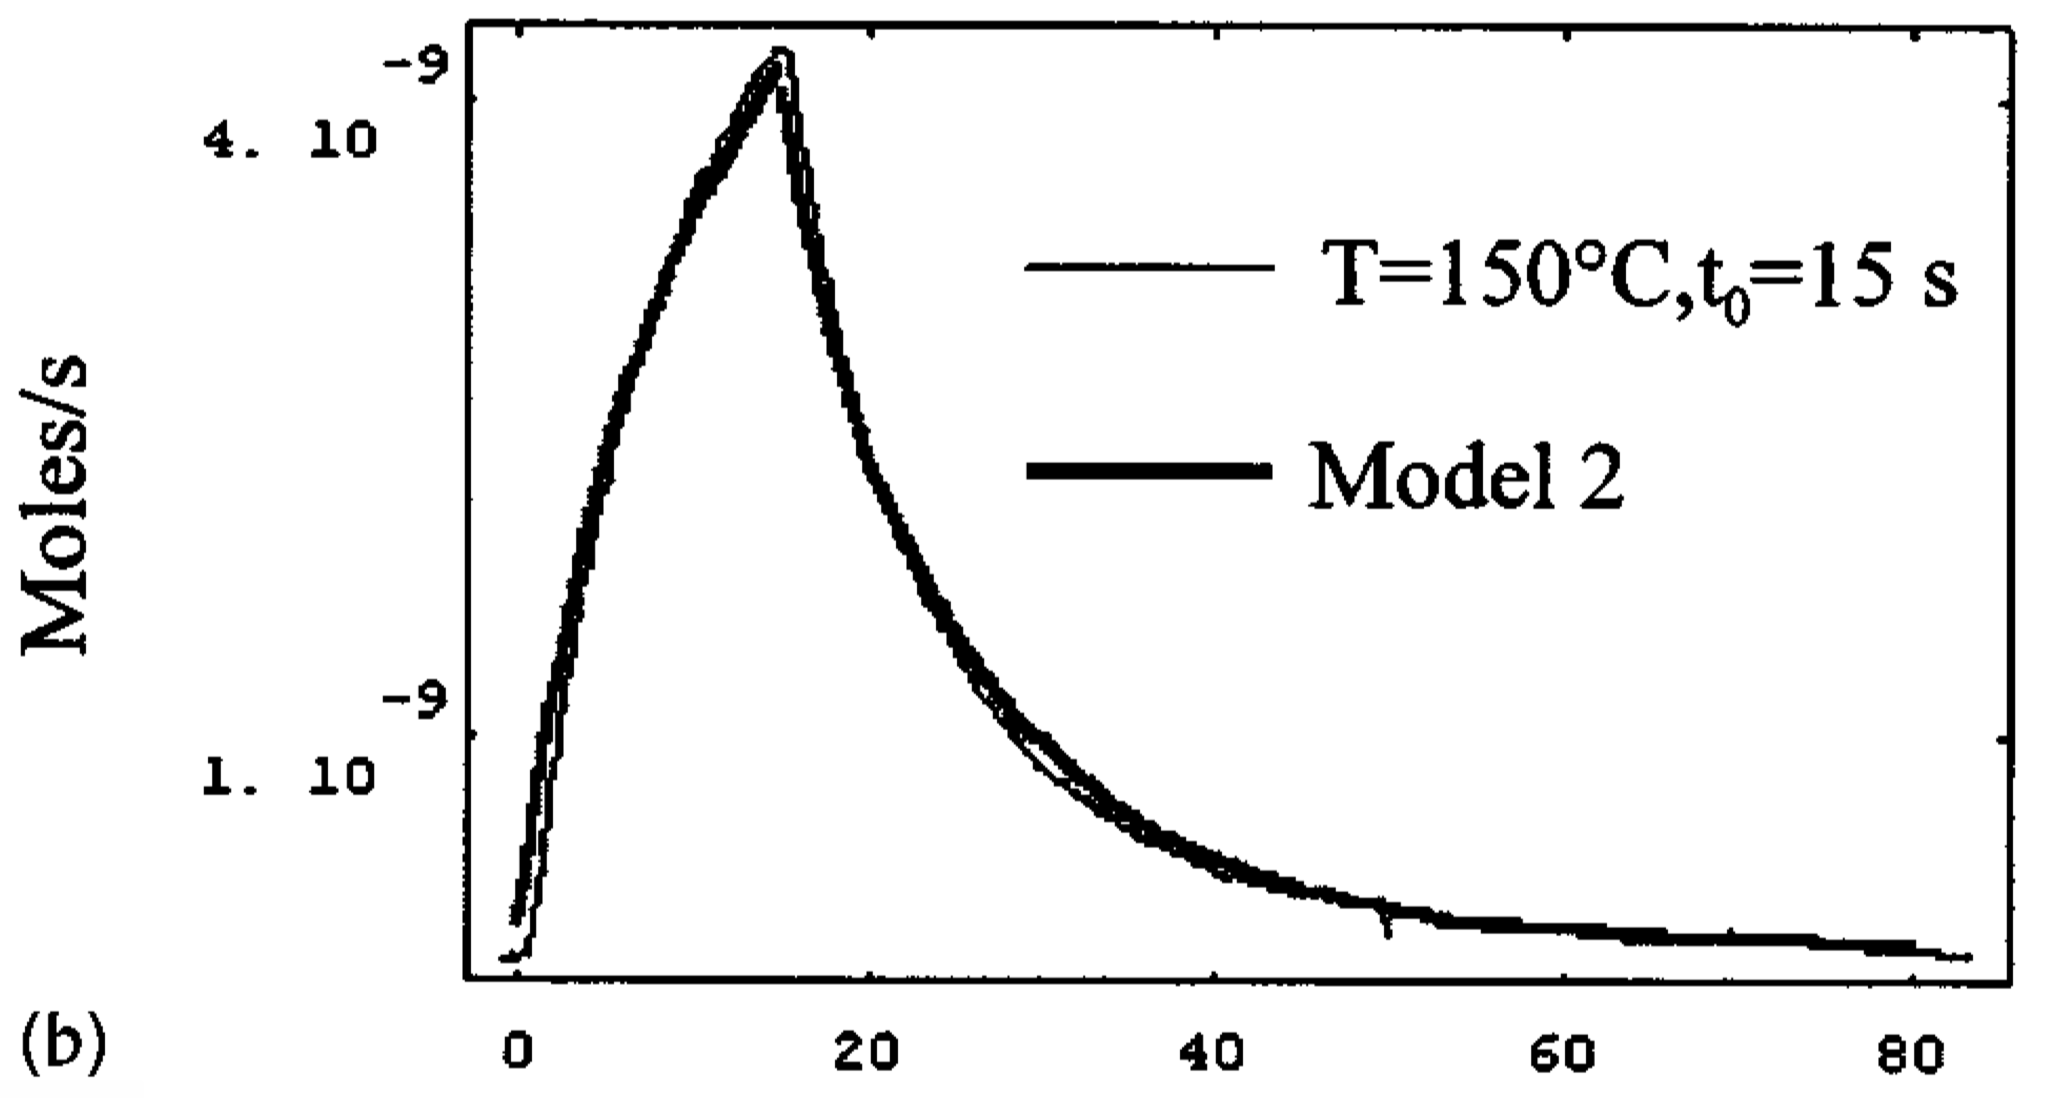
\includegraphics[width=\linewidth]{150_15.png}
	\end{minipage}
	\caption{Экспериментальная зависимость скорости выхода мономера из слоя ПММА при экспонировании ионным лучом и результаты моделирования, полученные в работе для температур 135$^\circ$C и 150$^\circ$C~\cite{Fragala_3_diffusion}}
\end{figure}

\begin{table}[h]
	\begin{center}
	\caption{Константы процессов инициирования активного центра и деполимеризации и коэффициенты диффузии, полученные в работе~\cite{Fragala_3_diffusion} для различных температур.}
	\begin{tabular}{lc rc rc r}
		\hline \hline
		Температура, $^\circ$C & \hspace{4em} & $K_i \beta$, с$^{-1}$ & \hspace{1em} & $K_p$, с$^{-1}$ & \hspace{1em} & $D$, см$^2$с$^{-1}$ \\ \hline
		135 & \hspace{4em} & $7 \times 10^{-4}$ & \hspace{1em} & 90 & \hspace{1em} & $2 \times 10^{-10}$ \\  
		150 & \hspace{4em} & $1.85 \times 10^{-3}$ & \hspace{1em} & 100 & \hspace{1em} & $3.5 \times 10^{-10}$ \\
		160 & \hspace{4em} & $1.6 \times 10^{-3}$ & \hspace{1em} & 100 & \hspace{1em} & $1.1 \times 10^{-9}$ \\
		170 & \hspace{4em} & $3.2 \times 10^{-3}$ & \hspace{1em} & 120 & \hspace{1em} & $1.2\times10^{-9}$ \\
		185 & \hspace{4em} & $3.1 \times 10^{-3}$ & \hspace{1em} & 300 & \hspace{1em} & $2.1\times10^{-9}$ \\ \hline \hline
	\end{tabular}
	\label{table:Ki_Kp_D}
	\end{center}
\end{table}
